\documentclass[varwidth=true, border=2pt]{standalone}
\usepackage{tkz-euclide}

\begin{document}
\usetkzobj{all}
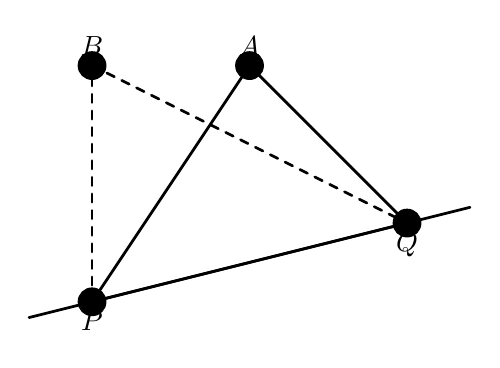
\begin{tikzpicture}
    \tkzSetUpPoint[shape=circle,size=10,color=black,fill=black]
    \tkzSetUpLine[line width=1]
    \tkzDefPoints{0/0/P, 4/1/Q, 2/3/A, 0/3/B}

    \tkzDrawSegments(P,Q Q,A A,P)
    \tkzDrawSegments[dashed](P,B B,Q)
    \tkzDrawLine(P,Q)

    \tkzDrawPoints(P,Q,A,B)
    \tkzLabelPoint[below](P){$P$}
    \tkzLabelPoint[below](Q){$Q$}
    \tkzLabelPoint[above](A){$A$}
    \tkzLabelPoint[above](B){$B$}
\end{tikzpicture}
\end{document}
